% \documentclass{beamer}
\documentclass[handout]{beamer}

\usetheme[secheader]{Boadilla}

\usepackage[english]{babel}
% \usepackage[italian, english]{babel}
\usepackage[utf8]{inputenc} % needed for bibtex
\usepackage{mathrsfs}
\usepackage{amsthm}
\usepackage{amsmath}
\usepackage{amssymb}
\usepackage{mathtools}
%\usepackage{nccmath} % mfracf
%\mathbb needs amsfonts or amssymb
\usepackage{amsfonts}
\usepackage{bm} % bold symbols math

% \usepackage[overload]{empheq} % left\{ for align % no crash kile ?
\usepackage{cases}
% \usepackage[usenames,dvipsnames]{xcolor} % before tikz, options for more colors
% \definecolor{light-gray}{gray}{0.95}

\usepackage{booktabs}
\usepackage{caption}
\usepackage{subfig}
% \captionsetup[figure]{width=.85\textwidth}
\captionsetup[subfigure]{margin=0.5cm}

%%%%%%%%%%%%%%%%%%%%%%%%%%%%%%%%%%%%%%%%%%%%%%%%%%% color
%\usepackage{color}
\usepackage{xcolor}
\definecolor{ao(english)}{rgb}{0.0, 0.5, 0.0}
\definecolor{blue-violet}{rgb}{0.54, 0.17, 0.89}
\definecolor{brightpink}{rgb}{1.0, 0.0, 0.5}

\definecolor{deepjunglegreen}{rgb}{0.0, 0.29, 0.29}
\definecolor{darkpowderblue}{rgb}{0.0, 0.2, 0.6}
% \definecolor{bookColor}{cmyk}{1 , 1  , 0   , 0}  % 0.90\% of black
% \color{bookColor}
%%%%%%%%%%%%%%%%%%%%%%%%%%%%%%%%%%%%%%%%%%%%%%%%%%%%



\usepackage{tikz}
\usetikzlibrary{matrix}
\usetikzlibrary{positioning}
% set arrows as stealth fighter jets
\tikzset{>=stealth}
% bezier
\usetikzlibrary{decorations.pathreplacing}
\tikzset{%
  show curve controls/.style={
    postaction={
      decoration={
        show path construction,
        curveto code={
          \draw [blue] 
            (\tikzinputsegmentfirst) -- (\tikzinputsegmentsupporta)
            (\tikzinputsegmentlast) -- (\tikzinputsegmentsupportb);
          \fill [red, opacity=0.5] 
            (\tikzinputsegmentsupporta) circle [radius=.5ex]
            (\tikzinputsegmentsupportb) circle [radius=.5ex];
        }
      },
      decorate
}}}
\tikzstyle{mybox} = [draw=gray, fill=light-gray, very thick,
    rectangle, rounded corners, inner sep=10pt, inner ysep=20pt]
\tikzstyle{mytitle} =[fill=gray, text=white]

% plots
\usepackage{pgfplots}


% \usepackage{hyperref}
% \hypersetup{pdftex,colorlinks=true,allcolors=blue}
% \usepackage{hypcap}
% \usepackage{etoolbox}
% 
% \usepackage{csquotes}
% %\usepackage[autostyle, italian=guillemets]{csquotes}
% 
% % \usepackage[chapter]{placeins} % floatbarrier
% 
\usepackage[backend=biber, style=alphabetic]{biblatex}
\addbibresource{../tex/sources.bib}
\DeclareFieldFormat[article]{title}{\textit{#1}}

% 
% \numberwithin{equation}{section}
% 
% \theoremstyle{definition}
% \newtheorem{definition}[subsection]{Definition}
% \theoremstyle{plain}
% \newtheorem{theorem}[subsection]{Theorem}
% \theoremstyle{plain}
% \newtheorem{corollary}[subsection]{Corollary}
% \theoremstyle{plain}
% \newtheorem{proposition}[subsection]{Proposition}
% \theoremstyle{plain}
% \newtheorem{remark}[subsection]{Remark}
% \theoremstyle{plain}
% \newtheorem{lemma}[subsection]{Lemma}
% \theoremstyle{plain}
% \newtheorem{example}[subsection]{Example}
% 
% \theoremstyle{plain}
% \newtheorem{assumption}[subsection]{Assumption}
% \theoremstyle{plain}
% \newtheorem{problem}[subsection]{Problem}

\DeclareMathOperator{\divergence}{div}
\DeclareMathOperator{\curl}{curl}
\DeclareMathOperator{\real}{Re}
\DeclareMathOperator{\imag}{Im}

\renewcommand{\i}{\textup{i}}
\let\phi\varphi
\let\epsilon\varepsilon

\newcommand{\upin}{\textup{ in }}
\newcommand{\upon}{\textup{ on }}

%%%%%%%%%%%%%%%%%%%%%%%%%%%%%%
\usepackage{amssymb,tikz}

\newcommand{\mysetminusD}{\hbox{\tikz{\draw[line width=0.6pt,line cap=round] (3pt,0) -- (0,6pt);}}}
\newcommand{\mysetminusT}{\mysetminusD}
\newcommand{\mysetminusS}{\hbox{\tikz{\draw[line width=0.45pt,line cap=round] (2pt,0) -- (0,4pt);}}}
\newcommand{\mysetminusSS}{\hbox{\tikz{\draw[line width=0.4pt,line cap=round] (1.5pt,0) -- (0,3pt);}}}

\newcommand{\mysetminus}{\mathbin{\mathchoice{\mysetminusD}{\mysetminusT}{\mysetminusS}{\mysetminusSS}}}
%%%%%%%%%%%%%%%%%%%%%%%%%%%%%%%%%%


% \usepackage{environ}
% \NewEnviron{mybox}{%
% \begin{center}
% \colorbox{light-gray}{\color{black}\parbox{\textwidth}{%
% % \fcolorbox{gray}{light-gray}{
% \BODY
% }}
% \end{center}
% }
% 
% \usepackage{fancyhdr}
% \newcommand{\fncyblank}{\fancyhf{}}
%%%%%%%%%%%%%%%%%%%%%%%%%%%%%%%%%%%%%%%%%%%% abstract already defined
% \newenvironment{abstract} %
% {\cleardoublepage\fncyblank\null\vfill\begin{center} %
% \bfseries\abstractname\end{center}} %
% {\vfill\null}
%%%%%%%%%%%%%%%%%%%%%%%%%%%%%%%%%%%%%%%%%%%%%%%%%%%%%%%%%%%%%%%%%%%%%%%%%
\title{The Boundary Integral Method}
\author{Giacomo Milan}
\date{14 Settembre 2017}
%%%%%%%%%%%%%%%%%%%%%%%%%%%%%%%%%
\begin{document}
\begin{frame}
%  \maketitle
    \begin{center}
        \textsc{Politecnico di Milano}\\
%         Scuola di Ingegneria Industriale e dell'Informazione\\
        \vspace{1cm}
        \includegraphics[width=0.2\textwidth]{../tex/fig/logo_bw} \\
%         \small
%         \vspace{3cm}
%         Project of \\
%         \large
%         \textsc{Numerical Analysis for Partial Differential Equations}\\
%         \begin{flushright}
%         \normalsize
%          Prof.ssa Perotto
%         \end{flushright}
% %         \vspace{0.5cm}
%         \normalsize
%         Course of \\
%         \large
%         \textsc{Mathematical Engineering}
% %         
% % 
        \vspace{0.8cm}
        \Large
        \textsc{The Boundary Element Method}
        
%       \vspace{0.5cm}
%       Thesis Subtitle
        
%         \vspace{1.5cm}
        \begin{flushright}
        \small
        {Giacomo Milan\\ Matr. 841530}         
        \end{flushright}
        \normalsize
        \vfill
        Anno accademico 2016-2017
        
    \end{center}
\end{frame}
%%%%%%%%%%%%%%%
\begin{frame}
 \frametitle{Starting from an example}
We consider the Laplace equation in an open set $\Omega$ of class $C^2$
\begin{eqnarray}
 \Delta u = 0, & \textup{ in }\Omega,\label{eq:laplace-in}\\
 u = g, & \textup{ on }\partial\Omega.\label{eq:laplace-on}
\end{eqnarray}
\pause
The aim is to write the solution $u$ through {\color{blue}representation formulas}
in terms of its boundary data
\begin{center}
$u|_{\partial \Omega}$, $\partial_\nu u|_{\partial \Omega}$, $\Delta u$,
\end{center}
\pause
but in our problem
\begin{center}
 {\color{blue}$\partial_\nu u|_{\partial \Omega}$ = ?} is unknown
\end{center}

\end{frame}
%%%%%%%%%%%%%%%
\begin{frame}
 \frametitle{Representation Formula}
We generalize to the problem
\begin{equation}
Lu = f, \text{ in }\mathcal{D}'(\Omega).
\end{equation}
\pause
Let $\Phi(z,z_0)$ denote the {\color{blue}fundamental solution} which solves
\begin{equation}
\label{eq:fundamental-solution}
 L\Phi=\delta_{z_0},\quad\upin\mathcal{D}'(\mathbb{R}^m).
\end{equation}
\pause
% For the Laplace equation with $L=-\Delta$, it can be explicitly expressed as
% \begin{equation}
% \label{eq:definition-Phi-23}
%   \Phi(z,z_0)=
%   \left\{
%   \begin{aligned}
%    &\dfrac{1}{2\pi}\log\dfrac{1}{| z - z_0|}, && m=2, \\
%    &\dfrac{1}{4\pi}\dfrac{1}{| z  - z_0|}, && m=3.
%   \end{aligned}
%   \right.
% \end{equation}
% \begin{block}{Theorem}
\begin{theorem}[Green's Formula]
Let $\Omega$ be a domain of class $C^2$ (or even Lipschitz regular),
and $u \in C^2(\Omega)\cap C^1(\overline{\Omega})$,
then, by classical Green's formula,
there holds the following integral representation formula
\begin{equation}
  \label{eq:representation-formula}
  - u(z_0) = \int_\Omega\Delta u\,\Phi_{z_0}\,dz 
  + \int_{\partial \Omega}\big(u\, \partial_{\nu(z)} \Phi_{z_0}
  - \partial_\nu u\,\Phi_{z_0}\big)\,dz, \quad z_0 \in \Omega.
\end{equation}
\end{theorem}
% \end{block}
\end{frame}
%%%%%%%%%%%%%%%
% \begin{frame}
%  \frametitle{}
%  as the sum of two layer potentials defined on $\partial\Omega$.
% Given a density $\psi\in C(\partial \Omega)$, we define
% \begin{enumerate}
%   \item the \emph{single layer} potential
%    \begin{equation}
%     \mathcal{S}(\partial \Omega,\psi)(z_0)\coloneqq \int_{\partial \Omega} \Phi(z_0, z)\psi(z)\, dz,\quad z_0\in\mathbb{R}^m \backslash\partial \Omega, \label{eq:definition-single-layer}
%    \end{equation}
%   \item the \emph{double layer} potential
%    \begin{equation}
%     \mathcal{D}(\partial \Omega,\psi)(z_0)\coloneqq \int_{\partial \Omega} \partial_{\nu(z)}\Phi(z_0, z)\psi(z)\, dz,\quad z_0\in\mathbb{R}^m \backslash\partial \Omega. \label{eq:definition-double-layer}
%    \end{equation}
% \end{enumerate}
% These potentials are analytic in $\mathbb{R}^m\backslash\partial\Omega$,
% while along the boundary $\partial\Omega$ there hold the well known \emph{jump relations}, 
% which can be expressed through the integral operators 
% $S, K, K': C(\partial \Omega)\to C(\partial \Omega)$.
% \end{frame}
%%%%%%%%%%%%%%
\begin{frame}
 \frametitle{Integral Layer Potentials}
%  which can be expressed through the integral operators 
% $S, K, K': C(\partial \Omega)\to C(\partial \Omega)$.
\begin{definition}
 We denote by $S$, $K$  and $K'$ the following integral operators 
 defined on $C(\partial \Omega)$, where $\partial \Omega$ is of class $C^2$
 \begin{enumerate}
  \item  the single layer operator $ S: C(\partial \Omega) \to C(\partial \Omega)$
  \begin{equation}
  S\psi(z_0)\coloneqq\int_{\partial \Omega}\psi(z) \Phi(z_0,z)\,dz,\label{def:operator-S}
  \end{equation}
  \item  the double layer operator $ K:C(\partial \Omega) \to C(\partial \Omega)$
  \begin{align}
  & K\psi(z_0)\coloneqq\int_{\partial \Omega} \psi(z) \partial_{\nu(z)} \Phi(z_0, z) \,dz,
%   = \int_{\partial \Omega} \psi(z) \nabla_z\Phi(z_0, z)\cdot\nu(z) \,dz,
  \label{def:operator-K}
%   \\
%   & K'\psi(z_0)\coloneqq\int_{\partial \Omega} \psi(z) \partial_{\nu(z_0)} \Phi(z_0, z) \,dz =
%   \int_{\partial \Omega} \psi(z) \nabla_{z_0}\Phi(z_0, z)\cdot\nu(z_0) \,dz.\label{def:operator-K'}
  \end{align}
  \item $K'$ the adjoint operator of $K$.
 \end{enumerate}
\end{definition}
\end{frame}
%%%%%%%%%%%%%%
\begin{frame}
 \frametitle{Jump Relations}
 There hold the following limits (see \cite{kress:book}, \cite{salsa:book})
  \begin{enumerate}
  \item the single layer is continuous and 
  \begin{subequations}
  \begin{align}
   \mathcal{S}^+(z)&=\mathcal{S}^-(z)&&\quad z\in\partial \Omega,\label{eq:single-pm-0}\\
%    \mathcal{S}^\pm(z) &\coloneqq\lim_{h\to 0^\pm}\mathcal{S}(z+h\nu(z)) = S\psi(z)=\int_{\partial \Omega}\psi(y)\Phi(z,y)\,dy \quad z\in\partial \Omega, \label{eq:single-pm-0}\\
   \partial_\nu\mathcal{S}^\pm(z) &
%    \coloneqq \lim_{h\to0^\pm} \nabla\mathcal{S}(z+h\nu(z))\cdot\nu(z) 
   =  K'\psi(z) \,\mp\,\dfrac{1}{2}\psi(z) &&\quad z\in\partial \Omega,\label{eq:single-pm-1}
  \end{align}
 \end{subequations}
 \item the double layer can be continuously extended from $\Omega$ to $\overline{\Omega}$, from $\mathbb{R}^m\backslash \overline{\Omega}$ to $\mathbb{R}^m\backslash \Omega$, and
  \begin{subequations}
  \begin{align}
   \mathcal{D}^\pm(z) &= K\psi(z) \pm\dfrac{1}{2}\psi(z)\quad&& z\in\partial \Omega, \label{eq:double-pm-0}\\
   \partial_\nu\mathcal{D}^+(z) &= \partial_\nu\mathcal{D}^-(z) \quad &&z\in\partial \Omega. \label{eq:double-pm-1}
  \end{align}
  \end{subequations}
 \end{enumerate}
\end{frame}
%%%%%%%%%%%%%%%
\begin{frame}
 \frametitle{Boundary Integal Equations}
 We go back to Laplace problem \eqref{eq:laplace-in} with boundary data
%  , it's convenient to represent the 
% solution in different ways, according with the nature of boundary conditions
\begin{align}
  u = g, & \textup{ on }\partial\Omega, \quad \Rightarrow \quad u = \mathcal{D}(\partial\Omega;\, \psi), \label{eq:bc-lap-dir}\\
  \partial_\nu u = g, & \textup{ on }\partial\Omega, \quad \Rightarrow \quad u = \mathcal{S}(\partial\Omega;\, \psi), \label{eq:bc-lap-neum}
\end{align}
\pause
which respectively yield to equations
\begin{align}
 (K - 0.5 I)\psi &= g,\label{eq:bie-dir}\\
 (K' + 0.5 I)\psi &= g.\label{eq:bie-neum}
\end{align}
with a Fredholm operator of the second kind {\color{blue}$B - I$}, $B$ compact
\end{frame}
%%%%%%%%%%%%%%%
\begin{frame}
 \frametitle{Boundary Element Method}
 We consider the discretization
  \begin{align}
  \psi\in X:\quad A\psi&=f,\quad\textup{ in }Y,\\
  \psi\in {\color{blue}X_n}:\quad A\psi&=f,\quad\textup{ in }Y.
  \end{align}
% and we solve it for $u$ belonging to the finite dimensional 
% subspace $X_n\subset X$.
\pause
We denote by $\{\psi_j\}_{i=0}^m$ the finite basis of $X_n$, 
therefore
% the integral equations \eqref{eq:bie-dir} and \eqref{eq:bie-neum} are reduced to
\begin{equation}
 \psi=\sum_{j=0}^m\psi_j\alpha_j\Rightarrow\sum_{j=0}^m(A\psi_j) \alpha_j = f \upon \partial\Omega.\label{eq:directlinear}
\end{equation}
\end{frame}
%%%%%%%%%%%%%%%
\begin{frame}
 \frametitle{Boundary Element Method}
 The second discretization is called {\color{blue}projection method}(see \cite{kirsch:book})
  \begin{align}
  \psi\in {X_n}:\quad A\psi&=f,\quad\textup{ in }Y, \\
  \psi\in {X_n}:\quad {\color{blue}Q_n}A\psi&={\color{blue}Q_n}f,\quad\textup{ in }{\color{blue}Y_n}.
  \end{align}
\pause
The most popular choice is the {\color{blue}collocation method}, which has the advantage of 
performing only one integration, then
\begin{center}
 we denote by $z_i = c(\tau_i)$ the collocation nodes
\end{center}
\begin{equation}
 \sum_{j=0}^m{\color{blue-violet}(A\psi_j)(z_i)} \alpha_j = {\color{brightpink}f(z_i)}, 
 \quad \textup{ or }\quad \sum_{j=0}^m{\color{blue-violet}A_{ij}}\alpha_j = {\color{brightpink}\beta_i}, 
 \quad i=0,\dots,m.\label{eq:bie-collocated}
\end{equation}
Further details on \cite{brebbia:book}, \cite{brebbia:book-progress}.
\end{frame}
%%%%%%%%%%%%%%%
\begin{frame}
 \frametitle{Pros and Cons}
 We list main advantages
%  of the formulation of the problem through boundary integrals, 
% instead of using for instance the discretization of the variational formulation with the FEM.
\begin{exampleblock}{}
\begin{enumerate}[<+->]
 \item the discretization of the boundary instead of a domain is less expansive;
%  The expression of the solution reduces to a boundary integral,
%  and allows not to consider the full domain. The discretization of a curve, instead of an area 
%  in two dimension (or a surface instead of a volume in three dimension), is less expensive.
 \item we can deal with unbounded regions in exterior problems;
%  , as easily as we do with bounded regions.
 \item for smooth data the rate of convergence can be very high, even exponential.
\end{enumerate}
\end{exampleblock}
On the other end, we present the main disadvantages
\begin{alertblock}{}
\begin{enumerate}[<+->]
 \item it requires the knowledge of the fundamental solution; 
 \item we can not solve 
 differential problem with non constant parameters;
 \item singularities of the integral kernels 
  requires a convergent quadrature method;
 \item boundaries with corners.
%  where the unknown densities are singular. The quadrature rule requires a more 
%  careful collocation of the nodes.
\end{enumerate}
\end{alertblock}
\end{frame}

%%%%%%%%%%%%%%%
\begin{frame}
 \frametitle{Parametrization of the Geometry}
Let $\partial\Omega$ be a curve 
in $\mathbb{R}^2$ of class $C^2$ parametrized by
\begin{equation}
c(t):[0,2\pi]\to\mathbb{R}^2,
\end{equation}
\begin{center}
let $\mathcal{P}_n = \{[\tau_k^{(n)},\tau_{k+1}^{(n)}]\}_{k=0}^{2n-1}$
be a partition of 
the interval $[0, 2\pi]$
\end{center}
% , with equidistant nodes $\tau_k^{(n)}=k\pi/n$, 
% which defines a partition $\mathcal{E}_n = \{E_k\}_{k=0}^{2n-1}$ of the boundary 
% $\partial \Omega=\bigcup E_k$, with $E_k \coloneqq c([\tau_k, \tau_{k+1}])$.
\begin{center}
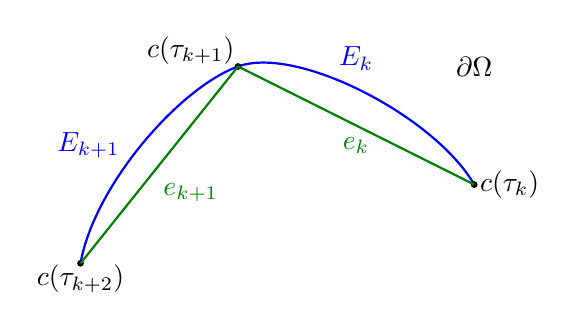
\begin{tikzpicture}
\draw [thick, blue] (-2, -1) 
  .. controls ++(80:1) and ++(20:-0.8) .. (0, 1.5)
  .. controls ++(20:0.8) and ++(120:1) .. (3, 0);
\node at (-2,-1.2){$c(\tau_{k+2})$};
\node at (-0.6,1.7){$c(\tau_{k+1})$};
\node at (3.45,0){$c(\tau_{k})$};
\node at (1.5,0.5){\color{ao(english)}$e_k$};
\node at (1.5,1.6){\color{blue}$E_k$};
\node at (-0.6,-0.1){\color{ao(english)}$e_{k+1}$};
\node at (-1.9,0.5){\color{blue}$E_{k+1}$};
\node at (3.0,1.5)(boundary){$\partial \Omega$};

\draw [fill] (-2,-1) circle [radius=1pt];
\draw [fill] (0,1.5) circle [radius=1pt];
\draw [fill] (3,0) circle [radius=1pt];
\draw [thick, ao(english)] (-2,-1)--(0, 1.5);
\draw [thick, ao(english)] (3,0)--(0, 1.5);
\end{tikzpicture}
\hspace*{-1cm}
\begin{tikzpicture}
\draw [] (-1,0)--(1, 0);
\draw [fill] (-1,0) circle [radius=1pt];
\draw [fill] (0,0) circle [radius=1pt];
\draw [fill] (1,0) circle [radius=1pt];
\node at (-1,-0.2){$\tau_{k}$};
\node at (0,-0.2){$\tau_{k+1}$};
\node at (1,-0.2){$\tau_{k+2}$};

\node (x2) at (-4,2.5){$ $};
\node (x1) at (0,0.5){$ $};

\draw[->] (x1) to [out=90,in=0] node[above,midway]{$c$}(x2);
\end{tikzpicture}
\end{center}

\end{frame}
%%%%%%%%%%%%%%%
\begin{frame}
\frametitle{Finite Element Spaces}
We can consider two similar discrete spaces.
\begin{definition}
The finite element space of continuous, piecewise polynomial functions of degree $r$, 
defined on {\color{blue}$\partial\Omega_h$}
\begin{equation}
 X^r_h \coloneqq \{v_h\in C^0(\partial\Omega_h):v_h|_{e_k} \in \mathbb{P}^r,\, \forall e_k\in \partial\Omega_h\}.
\end{equation}
\end{definition}
We can associate to $X^r_h$ a collection of {\color{blue}nodes} $z_i$ and 
a {\color{blue}lagrangian basis}
denoted by $\{\psi_j\}_{i=0}^m$.
\begin{definition}
The space of finite element functions $v(c(t))$ on $[0,2\pi]$, 
defined on {\color{blue}$\partial\Omega$}
\begin{equation}
 X^r_n \coloneqq \{v_n\in C^0(\partial\Omega):v_n(c(t))|_{I_K} \in \mathbb{P}^r,\, \forall I_K\in \mathcal{P}_n\}.
\end{equation}
\end{definition}
\end{frame}
%%%%%%%%%%%%%%%
\begin{frame}
 \frametitle{Quadrature}
We apply a quadrature rule to $A_{ij} = A\psi_j(z_i)$
\begin{equation}
 A_{ij} = A\psi_j(z_i) = \int_{\partial\Omega}\partial_{\nu(z)}\Phi(z_i, z)\psi_j(z)\,dz  - \frac{1}{2}\psi_j(z_i).
\end{equation}
which has a continuous kernel for a $C^2$ boundary.
\pause
\par
We report the quadrature points and weights in the software
FreeFem++ implemented in the finite element spaces
denoted by P0, P1, P2.
% 9.6884482205476277804
% wh
% 9.682030647015111
\begin{center}
\begin{tabular}{lccc}
\toprule
 qfe & point in $[z_i, z_{i+1}](=t)$ & 
 $\omega$ & $r$(exact on $\mathbb{P}^r$)\\
\midrule
qf1pE & $1/2$ &  $|z_iz_{i+1}|$ & 1\\
qf2pE & $(1\pm\sqrt{1/3})/2$ &  $|z_iz_{i+1}|/2$ & 3\\
qf1pElump & $\{0, 1\}$ & $|z_iz_{i+1}|/2$ & 1\\
\bottomrule
\end{tabular}
\end{center}
\end{frame}
%%%%%%%%%%%%%%%
\begin{frame}
 \frametitle{Piecewise quadratic solution}
 We consider $\psi\in X^2_h$ on $\partial\Omega_h$
\begin{center}
\begin{figure}
% \subfloat[][\emph{Linear sampling method for $\alpha=\mathrm{1e}{-10}$}.]
\centering
{
\includegraphics[width=.40\textwidth]{../tex/fig/geometry_qf2}
}
\caption{\emph{Discretized boundary $\partial\Omega_h$, with red '*' as collocation nodes of $X^2_h$, 
corresponding to vertices and midpoints of the segments, and with blue 'o' as quadrature nodes, as in the 
previous table}.}
\label{fig:qf2}
\end{figure}
\end{center}
\end{frame}
%%%%%%%%%%%%%%%
% ``‘qf1pElump'''
% \begin{frame}
%  \frametitle{Examples}
% Therefore the choice of ``qf1pElump'' for $X^1_h$ yields to (by $\psi_j(z_k) = \delta_{jk}$)
% \begin{equation}
% \label{eq:Aij-X1h}
%  A_{ij} = \frac{1}{2}\big(|z_jz_{j-1}| + |z_jz_{j+1}|\big)\partial_{z}\Phi(z_i,z_j)\cdot \nu(z_j) - \frac{1}{2} \delta_{ij}.
% \end{equation}
% or ``qf2pE'' for $X^2_h$ to
% \begin{equation}
% \label{eq:Aij-X1h}
%  A_{ij} = \frac{1}{2}\big(|z_jz_{j-1}| + |z_jz_{j+1}|\big)\partial_{z}\Phi(z_i,z_j)\cdot \nu(z_j) - \frac{1}{2} \delta_{ij}.
% \end{equation}
% or ``qf1pElump'' for $X^1_n$ to
% \begin{equation}
% \label{eq:Aij-X1h}
%  A_{ij} = |c'(\tau_j)|\partial_{z}\Phi(z_i,z_j)\cdot \nu(z_j) - \frac{1}{2} \delta_{ij}.
% \end{equation}
% \end{frame}
%%%%%%%%%%%%%%%
% \begin{frame}
%  \frametitle{}
%  \begin{center}
% \begin{figure}
% % \subfloat[][\emph{Linear sampling method for $\alpha=\mathrm{1e}{-10}$}.]
% {
% \includegraphics[width=.34\textwidth]{../tex/fig/ploterrorqf210}
% }
% {
% \includegraphics[width=.30\textwidth]{../tex/fig/ploterrorqf250}
% }
% {
% \includegraphics[width=.30\textwidth]{../tex/fig/ploterrorqf250_zoom}
% }
% % \subfloat[][\emph{Factorization method}.]
% % {
% % \includegraphics[width=.48\textwidth]{../tex/fig/one_ellipse_fm_ellipse0}
% % }
% \caption{\emph{Error difference $u_h - u$ computed with the space $X^2_h$, 
% using $n=10$ in the first image, and $n=50$ in the second, as can be observed with by the colorbars, 
% for an elliptic domain $\Omega$. The third image is the zoomed picture of the second to 
% evidence that in BEM the error is greater on the integration boundary.}}
% \label{fig:ploterrorqf2}
% \end{figure}
% \end{center}
% \end{frame}
%%%%%%%%%%%%%%%
\begin{frame}
 \frametitle{}
\begin{center}
\begin{figure}
{
\includegraphics[width=.40\textwidth]{../tex/fig/plotellipse_qf2_dir_int_50}
}
{
\includegraphics[width=.40\textwidth]{../tex/fig/plotellipse_qf2_dir_int_50_exact}
}
\\
\centering
{
\includegraphics[width=.40\textwidth]{../tex/fig/plotellipse_qf2_dir_int_50_err}
}
\caption{Approximation $u_h$, exact $u$, and $u_h - u$, for the Laplace eq. 
with Dirichlet data, with $n=50$ nodes.}
\label{fig:ellipse_qf2_50}
\end{figure}
\end{center}
\end{frame}
%%%%%%%%%%%%%%%
\begin{frame}
 \frametitle{}
\begin{center}
\begin{figure}
{
\includegraphics[width=.40\textwidth]{../tex/fig/plotellipse_qf2_dir_int_150}
}
{
\includegraphics[width=.40\textwidth]{../tex/fig/plotellipse_qf2_dir_int_150_exact}
}
\\
\centering
{
\includegraphics[width=.40\textwidth]{../tex/fig/plotellipse_qf2_dir_int_150_err}
}
\caption{Approximation $u_h$, exact $u$, and $u_h - u$, for the Laplace eq. 
with Dirichlet data, with $n=150$ nodes.}
\label{fig:ellipse_qf2_150}
\end{figure}
\end{center}
\end{frame}
%%%%%%%%%%%%%%%
%%%%%%%%%%%%%%%%
\begin{frame}
 \frametitle{Logarithmic Singularity}
The fundamental solutions
of the Laplace equation and the Helmholtz equation have a {\color{blue}logarithmic 
singularity}
% with $z=c(\tau)$, $z_0=c(t)$, both belonging to $\partial\Omega$
\begin{align}
 L(t,\tau)
 \coloneqq
%  &\frac{1}{2\pi}\frac{1}{|c(t)-c(\tau)|}\frac{c(t)- c(\tau)}{|c(t)-c(\tau)|}
%  \cdot \nu(c(\tau))|c'(\tau)|\\
%  =
 &L_1(t,\tau)\ln\Big(4\sin^2\frac{t-\tau}{2}\Big)+L_2(t,\tau),
 \textup{ kernel of } K'
 \label{eq:def-kernel-L}\\
 M(t,\tau)
 \coloneqq
 &M_1(t,\tau)\ln\Big(4\sin^2\frac{t-\tau}{2}\Big)+M_2(t,\tau),
 \textup{ kernel of } S
 \label{eq:def-kernel-M}
\end{align}
% \begin{equation}
% \label{eq:def-kernel-M}
%  M(t,\tau)\coloneqq-\frac{1}{2\pi}\ln|c(t)-c(\tau)|=M_1(t,\tau)\ln\Big(4\sin^2\frac{t-\tau}{2}\Big)+M_2(t,\tau),
% \end{equation}

where all $L_1(t,\tau)$, $L_2(t,\tau)$, $M_1(t,\tau)$, $M_2(t,\tau)$ turn out
to be continuous and bounded (analytic) (see \cite{colton-kress:book}).
\pause
\par
\begin{lemma}
The {\color{blue} trigonometric interpolation} of the integrand can be computed
by the orthogonality relations
(see Lemma 8.21 contained in \cite{kress:book}),
\begin{equation}
 \frac{1}{2\pi}\int_0^{2\pi}\ln\Bigl(4\sin^2\frac{t}{2}\Bigr)e^{imt}\,dt=
 \begin{cases}
  0, & m=0, \\
  -1/|m|, & m=\pm1,\pm2,\dots
 \end{cases}
\end{equation}
\end{lemma}
\end{frame}
%%%%%%%%%%%%%%%
\begin{frame}
 \frametitle{Piecewise linear}
We can choose $\psi\in X^1_h$ on $\partial\Omega_h$
\begin{equation}
\label{eq:Aij-X1h}
 A_{ij} = {\color{blue}\frac{1}{2}\big(|z_jz_{j-1}| + |z_jz_{j+1}|\big)}\partial_{z}\Phi(z_i,z_j)\cdot \nu(z_j) - \frac{1}{2} \delta_{ij},
\end{equation}
\pause
or $\psi\in X^1_n$ on $\partial\Omega$
\begin{equation}
\label{eq:Aij-X1h}
 A_{ij} = {\color{blue}|c'(\tau_j)|}\partial_{z}\Phi(z_i,z_j)\cdot \nu(z_j) - \frac{1}{2} \delta_{ij}.
\end{equation}
\end{frame}
%%%%%%%%%%%%%%%
\begin{frame}
 \frametitle{Interior Laplace equation with Neumann data}
 \begin{center}
\begin{figure}
% \subfloat[][\emph{Linear sampling method for $\alpha=\mathrm{1e}{-10}$}.]
{
\includegraphics[width=.42\textwidth]{../tex/fig/cf_lap_neum_int_circle_exact}
}
{
\includegraphics[width=.42\textwidth]{../tex/fig/cf_lap_neum_int_circle}
}
\caption{\emph{Images of the exact solution $g$ on the left, and the approximation $u$ computed on the right,
for the interior Laplace problem with Neumann conditions}.}
\label{fig:cf_lap_neum_circle}
\end{figure}
\end{center}

\end{frame}
%%%%%%%%%%%%%%%
\begin{frame}
 \frametitle{Exterior Laplace equation with Neumann data}
\begin{center}
\begin{figure}
{
\includegraphics[width=.42\textwidth]{../tex/fig/cf_lap_neum_ext_circle_exact}
}
{
\includegraphics[width=.42\textwidth]{../tex/fig/cf_lap_neum_ext_circle}
}
\caption{\emph{Images of the exact solution $g$ on the left, and the approximation $u$ computed on the right,
for the exterior Laplace problem with Neumann conditions}.}
\label{fig:cf_lap_neum_circle_ext}
\end{figure}
\end{center}
Exterior BVPs
require a change in 
\eqref{eq:bie-dir} and \eqref{eq:bie-neum}, 
\begin{align}
 (K {\color{blue}+} 0.5 I)\psi &= g,\label{eq:bie-dir-ext}\\
 (K' {\color{blue}-} 0.5 I)\psi &= g.\label{eq:bie-neum-ext}
\end{align}
\end{frame}
%%%%%%%%%%%%%%%
\begin{frame}
 \frametitle{}
 In \cite{kress:book} are contained some estimates for the trapezoidal rule
applied to an analytic integrand $\psi(z)$, which yield to the estimate for $\psi\in X^1_n$
\begin{equation}
 \|Q_n\psi - \psi\|_{L^\infty(\partial\Omega)} \leq Ce^{-\sigma n}.
\end{equation}
% This method for the choice $X^1_n$ is a combination of collocation with quadrature as proved in \cite{kress:book}.
\begin{center}
\begin{figure}
% \subfloat[][\emph{Linear sampling method for $\alpha=\mathrm{1e}{-10}$}.]
% {
% \includegraphics[width=.25\textwidth]{fig/geometry_qf2}
% }
 \subfloat[][ ]
{
\includegraphics[width=.45\textwidth]{../tex/fig/convergence_dir_int_ellipse_qf2_infinity_power}
}
 \subfloat[][ ]
{
\includegraphics[width=.45\textwidth]{../tex/fig/convergence_dir_int_ellipse_exponential}
}
% \subfloat[][\emph{Factorization method}.]
% {
% \includegraphics[width=.48\textwidth]{fig/one_ellipse_fm_ellipse0}
% }
\caption{{\emph{Logarithmic plots of the $L^\infty(\Omega)$ error. In Figure (a) the error 
computed for $X^2_h$, according with a power law $n^{-2}$;
in Figure (b) the error 
computed for $X^1_n$, according with an exponential law.}}}
\label{fig:errorinfinty}
\end{figure}
\end{center}
\end{frame}
%%%%%%%%%%%%%%%
\begin{frame}
 \frametitle{The Helmoltz equation}
 We consider the Helmholtz equation 
in an open set $\Omega$ of class $C^2$
\begin{eqnarray}
 -\Delta u - k^2 u= 0, & \textup{ in }\Omega.\label{eq:helmholtz-in}
%  u = g, & \textup{ on }\partial\Omega.\label{eq:helmholtz-on}
\end{eqnarray}
We can end up with it every time we want to compute the time harmonic eigenmodes
$w(x,t)=e^{-i\omega t}u(x)$, with amplitude $u$, of an elastic membrane
which satisfies the wave equation $w_{tt} - c^2 \Delta w=0$. 
% In an homogeneous medium
% we can substitute the square of wave number $k^2$ in equation \eqref{eq:helmholtz-in}
% with $n k^2$, where $n=c_0^2/c^2$ is the refraction index and $c_0$ is the speed of sound.

\end{frame}
%%%%%%%%%%%%%%%
\begin{frame}
 \frametitle{The scattering problem}
 Let $\Omega$ be an open domain of class $C^2$, we denote by 
 \begin{itemize}[<+->]
  \item  $u_I$ the incident field, 
for example a plane wave $u_I = e^{-ik(\eta_1 x + \eta_2 y)}$,
  \item $u_S$ the scattered field,
 \end{itemize}
 \pause
 such that the
total field
\begin{equation}
 u=u_I + u_S\label{eq:def-total-fiels} 
\end{equation}
\pause
satisfies the Helmholtz equation in 
$\mathbb{R}^2\backslash\overline{\Omega}$, with Sommerfeld radiation 
conditions in $\mathbb{R}^2$ at infinity
\begin{align}
 \Delta u + k^2 u &= 0 \quad \upin \mathbb{R}^2\backslash\overline{\Omega},\\
 u(x)&=O(|x|^{-1}) \quad |x|\to \infty,\\
 \partial_r u - ik u &=o(|x|^{-1})\quad |x|\to \infty,   
\end{align}
\end{frame}
%%%%%%%%%%%%%%%%%%%%
\begin{frame}
\frametitle{The scattering problem}
and boundary conditions
\begin{enumerate}
 \item homogeneous Dirichlet boundary conditions for a \emph{sound-soft obstacle}
 \begin{equation}
  u = u_I + u_S= 0\quad\upon \partial \Omega,
 \end{equation}
 \item homogeneous Neumann boundary conditions for a \emph{sound-hard obstacle}
 \begin{equation}
  \partial_\nu u = \partial_\nu u_I + \partial_\nu u_S= 0\quad\upon \partial \Omega.
 \end{equation}
\end{enumerate}
\pause
The most convenient representation for the scattered field suggested in \cite{chen-zhou:book} is
\begin{equation}
 u_S(z_0)=\int_{\partial \Omega}\Big\{\partial_{\nu(z)}\Phi_z(z_0;k) -i\Phi_z(z_0;k)\Big\}\psi(z)\,dz.
\end{equation}
\end{frame}
%%%%%%%%%%%%%%%%%%%%%%
\begin{frame}
\begin{center}
\begin{figure}
% \subfloat[][\emph{Linear sampling method for $\alpha=\mathrm{1e}{-10}$}.]
{
\includegraphics[width=.30\textwidth]{../tex/fig/scatt_soft_inc_ellipse_10}
}
{
\includegraphics[width=.30\textwidth]{../tex/fig/scatt_soft_scatt_ellipse_10}
}
{
\includegraphics[width=.30\textwidth]{../tex/fig/scatt_soft_tot_ellipse_10}
}
\\
{
\includegraphics[width=.30\textwidth]{../tex/fig/scatt_soft_inc_ellipse_10_imag}
}
{
\includegraphics[width=.30\textwidth]{../tex/fig/scatt_soft_scatt_ellipse_10_imag}
}
{
\includegraphics[width=.30\textwidth]{../tex/fig/scatt_soft_tot_ellipse_10_imag}
}

% \subfloat[][\emph{Factorization method}.]
% {
% \includegraphics[width=.48\textwidth]{../tex/fig/one_ellipse_fm_ellipse0}
% }
\caption{\emph{Scattering problem, with homogeneous sound-soft conditions $u=0$. Images of the 
real and the imaginary parts
of the incident field $u_I$ (a plane wave with $\eta=(\cos\alpha,\, \sin\alpha)$ for $\alpha=\pi/4$), the scattered field 
$u_S$, and the total field $u=u_I + u_S$, respectively, for $k=10$}.}
\label{fig:scatt_soft_ellipse_10}
\end{figure}
\end{center}
% \begin{center}
% \begin{figure}
% % \subfloat[][\emph{Linear sampling method for $\alpha=\mathrm{1e}{-10}$}.]
% {
% \includegraphics[width=.30\textwidth]{../tex/fig/scatt_soft_inc_ellipse_10_imag}
% }
% {
% \includegraphics[width=.30\textwidth]{../tex/fig/scatt_soft_scatt_ellipse_10_imag}
% }
% {
% \includegraphics[width=.30\textwidth]{../tex/fig/scatt_soft_tot_ellipse_10_imag}
% }
% % \subfloat[][\emph{Factorization method}.]
% % {
% % \includegraphics[width=.48\textwidth]{../tex/fig/one_ellipse_fm_ellipse0}
% % }
% \caption{
% % \emph{Images of the imaginary part of the fields in 
% % Figure \ref{fig:scatt_soft_ellipse_10}}.
% }
% \label{fig:scatt_soft_ellipse_10_imag}
% \end{figure}
% \end{center}
\end{frame}
\begin{frame}[shrink=20]
\printbibliography % biber
\end{frame}
\begin{frame}
\begin{center}
\Large
 Thank you
\end{center}
\end{frame}


\end{document}
